\section{Istruzioni d'uso -- Cliente}

\subsection{Interfaccia principale e layout}
    \begin{figure}[H]
        \centering
        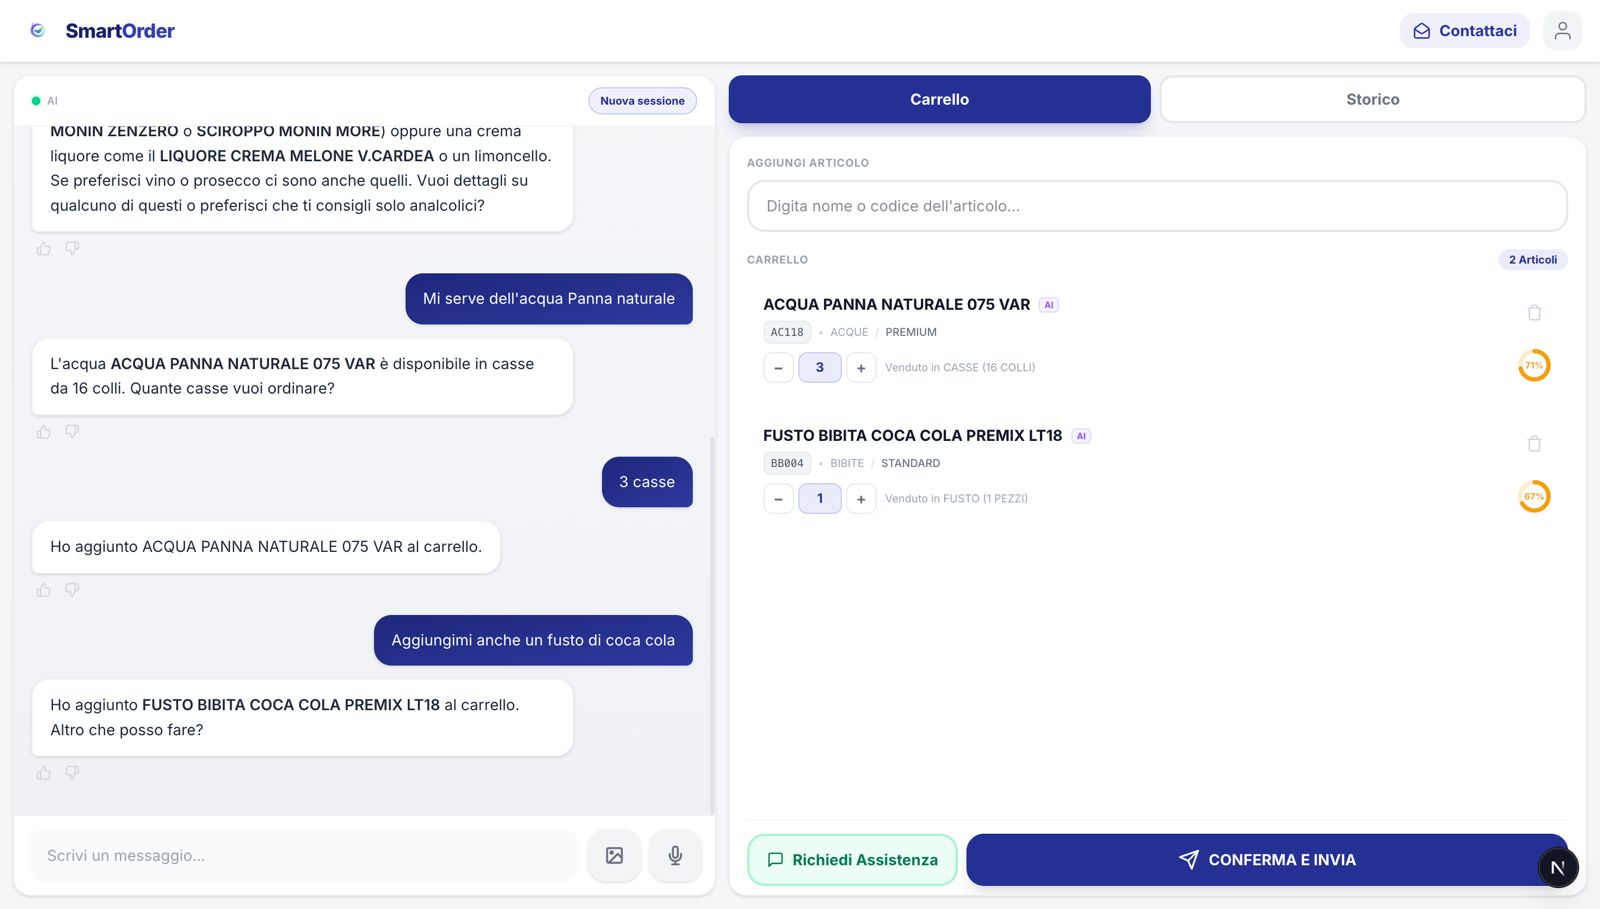
\includegraphics[width=0.7\textwidth]{Contenuti/immagini/schermata principale.jpeg}
        \caption{Schermata principale}
    \end{figure}

L'interfaccia Cliente si presenta con un layout responsive a tre pannelli:

\begin{itemize}
    \item \textbf{Pannello Chat} (45\% a sinistra, desktop): Area di conversazione con l'IA dove l'utente digita o detta i propri ordini.
    \item \textbf{Pannello Carrello/Storico} (55\% a destra, desktop): Alterna tra la visualizzazione del carrello e lo storico ordini tramite tab.
    \item \textbf{Tab Bar mobile} (schermo $< 768$px): Barra di navigazione inferiore con tre tab: Chat, Carrello, Storico.
\end{itemize}

In alto \`e presente la barra superiore con il logo e il pulsante per accedere all'area personale. Al primo accesso viene mostrata la schermata di login.

\subsection{Creazione di un ordine tramite chat}

Per creare un ordine utilizzando la chat con l'IA:

\begin{enumerate}
    \item \textbf{Identificazione}: Dopo aver effettuato il login, l'applicazione mostra la schermata principale. Se l'utente non \`e ancora stato identificato, viene richiesto di selezionare il proprio profilo cliente dall'overlay di autenticazione.
    \item \textbf{Composizione del messaggio}: Nella barra di input in fondo al pannello chat, digitare la richiesta in linguaggio naturale. Ad esempio: \texttt{Vorrei 5 confezioni di Pasta Barilla e 3 bottiglie di olio}. \`E possibile menzionare prodotti per nome, categoria o codice articolo.
    \item \textbf{Invio}: Premere Invio o cliccare sul pulsante di invio (icona freccia). Il messaggio appare nella chat con uno stile distintivo.
    \item \textbf{Risposta dell'IA}: L'IA elabora la richiesta e risponde confermando i prodotti identificati nel catalogo e le relative quantit\`a. Accanto a ciascun articolo proposto dall'IA compare un anello colorato che indica la confidenza della classificazione (verde = alta, rosso = bassa).
    \item \textbf{Aggiunta al carrello}: Se l'IA riconosce i prodotti nel catalogo, questi vengono aggiunti automaticamente al carrello. L'utente visualizza immediatamente gli articoli nel pannello di destra. La chat segnala eventuali articoli non trovati o non disponibili.
    \item \textbf{Feedback}: Sotto ogni risposta dell'IA compaiono due pulsanti: pollice in su (risposta utile) e pollice in gi\`u (segnala problema). Cliccando sul pollice in gi\`u si apre un modulo per selezionare un motivo e un commento opzionale.
\end{enumerate}

\subsection{Input vocale}

Per dettare un ordine usando la voce:

\begin{enumerate}
    \item \textbf{Attivazione}: Nella barra di input della chat, se il campo di testo \`e vuoto, cliccare sull'icona del microfono. Il browser richieder\`a l'autorizzazione per l'accesso al microfono.
    \item \textbf{Registrazione}: Il microfono si attiva e viene visualizzato un indicatore rosso pulsante con un visualizzatore a barre che mostra l'intensit\`a del suono captato in tempo reale.
    \item \textbf{Fine registrazione}: Cliccare sulla X per annullare la registrazione senza inviare, oppure cliccare sul pulsante di invio (freccia) per terminare e inviare automaticamente.
    \item \textbf{Trascrizione}: L'audio viene trascritto automaticamente tramite Whisper. Il testo riconosciuto appare come messaggio utente nella chat.
    \item \textbf{Errore}: Se il riconoscimento vocale non produce testo, l'IA risponde chiedendo di ripetere.
\end{enumerate}

\subsection{Ricerca e aggiunta manuale di prodotti}

Per cercare e aggiungere un prodotto manualmente (senza passare per la chat IA):

\begin{enumerate}
    \item \textbf{Campo di ricerca}: Nel pannello carrello, in alto, \`e presente il campo \texttt{Digita nome o codice dell'articolo}. Iniziare a digitare il nome o il codice del prodotto cercato.
    \item \textbf{Autocomplete}: Dopo 2 caratteri, vengono visualizzati i suggerimenti dal catalogo in tempo reale. Ogni suggerimento mostra: descrizione articolo, codice (badge), linea e famiglia.
    \item \textbf{Selezione}: Cliccare su un suggerimento per selezionare il prodotto. Viene visualizzata una card con il dettaglio del prodotto, comprensivo di unit\`a di misura e pezzi per confezione.
    \item \textbf{Quantit\`a}: Utilizzare i pulsanti \texttt{+} e \texttt{-} per impostare la quantit\`a desiderata, oppure digitare direttamente nel campo numerico.
    \item \textbf{Aggiunta}: Cliccare su \texttt{Aggiungi al carrello}. L'articolo appare nell'elenco sottostante con badge che ne indica l'origine manuale.
    \item \textbf{Annulla}: Cliccare sulla X in alto a destra della card per annullare la selezione.
\end{enumerate}

\subsection{Gestione del carrello}

Il pannello carrello mostra tutti gli articoli selezionati, distinti per origine:

\begin{itemize}
    \item \textbf{Articoli IA}: contrassegnati da badge \texttt{AI} di colore viola; includono l'anello di confidenza che indica l'attendibilit\`a della classificazione.
    \item \textbf{Articoli manuali}: aggiunti direttamente dall'utente; privi di badge.
\end{itemize}

Per ogni articolo nel carrello \`e possibile:

\begin{enumerate}
    \item \textbf{Modificare la quantit\`a}: Cliccare sul valore numerico della quantit\`a per trasformarlo in un campo modificabile. Impostare il nuovo valore e premere Invio, oppure usare i pulsanti \texttt{+} e \texttt{-}. Il carrello si aggiorna in tempo reale.
    \item \textbf{Rimuovere un articolo}: Cliccare sull'icona del cestino in alto a destra della riga dell'articolo. L'articolo viene rimosso immediatamente.
    \item \textbf{Articoli bloccati}: Se un articolo non \`e pi\`u disponibile al momento dell'invio dell'ordine, viene evidenziato in rosso con il messaggio \texttt{Articolo non pi\`u disponibile}. Rimuoverlo dal carrello per procedere.
\end{enumerate}

\subsection{Conferma e invio dell'ordine}

Per inviare l'ordine:

\begin{enumerate}
    \item \textbf{Revisione}: Verificare che tutti gli articoli nel carrello siano corretti e che le quantit\`a siano quelle desiderate.
    \item \textbf{Invio}: Cliccare sul pulsante viola \texttt{CONFERMA E INVIA} in basso a destra del pannello carrello. Se il carrello \`e vuoto, il pulsante \`e disabilitato.
    \item \textbf{Esito}: In caso di successo, il carrello viene svuotato, viene aperto automaticamente il pannello Storico e l'IA invia un messaggio di conferma nella chat. In caso di errore (articolo bloccato o non disponibile), viene visualizzato un messaggio di errore sopra il pulsante e l'articolo problematico viene evidenziato in rosso nel carrello.
\end{enumerate}


\subsection{Consultazione dello storico ordini}
    \begin{figure}[H]
        \centering
        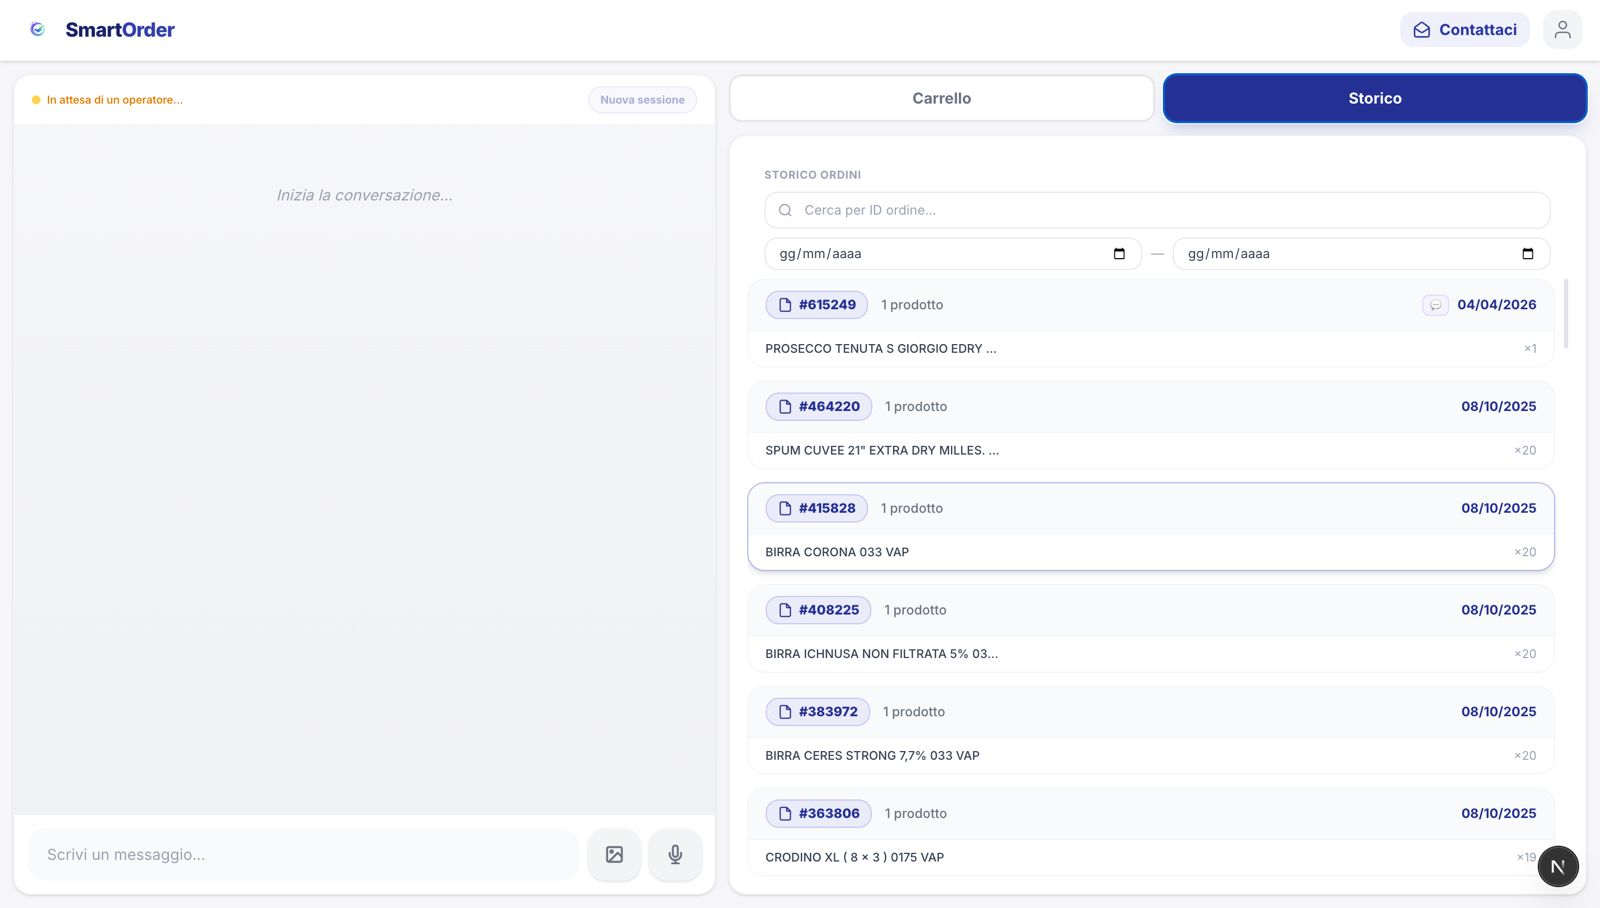
\includegraphics[width=0.7\textwidth]{Contenuti/immagini/storico cliente.jpeg}
        \caption{Visualizzazione dello storico degli ordini}
    \end{figure}

Per consultare gli ordini gi\`a inviati:

\begin{enumerate}
    \item \textbf{Accesso allo storico}: Sul desktop, cliccare sulla tab \texttt{Storico} in alto a destra nel pannello destro. Su mobile, selezionare la tab \texttt{Storico} nella barra inferiore.
    \item \textbf{Lista ordini}: Viene visualizzata la lista degli ordini, caricata con scroll infinito (i pi\`u recenti in alto). Ciascun ordine mostra la data e il conteggio degli articoli.
    \item \textbf{Filtri}:
    \begin{itemize}
        \item Campo di ricerca per ID ordine (ricerca debounced, attivata dopo 400~ms di inattivit\`a).
        \item Filtro per intervallo date: due campi data per data inizio e data fine.
        \item Pulsante X per cancellare tutti i filtri attivi.
    \end{itemize}
    \begin{figure}[H]
        \centering
        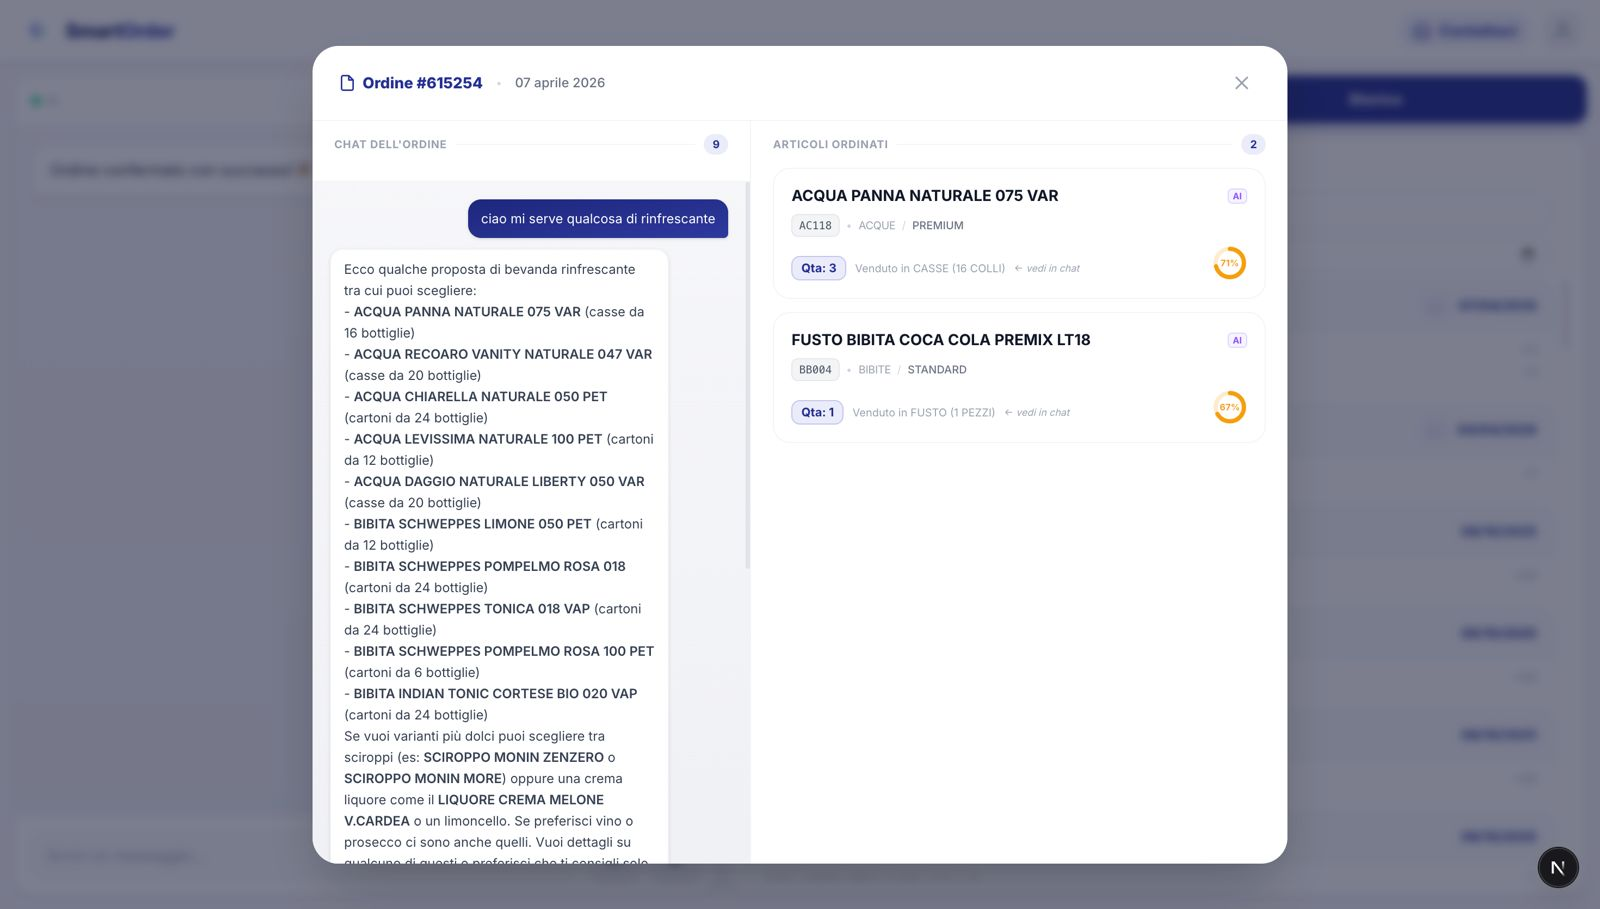
\includegraphics[width=0.7\textwidth]{Contenuti/immagini/dattagli ordine.jpeg}
        \caption{Dettagli ordine}
    \end{figure}
    \item \textbf{Dettaglio ordine}: Cliccare su un ordine per aprirne il dettaglio in un pannello modale. Il dettaglio mostra a sinistra la chat dell'ordine (con possibilit\`a di cliccare su un articolo per evidenziare il messaggio corrispondente nella chat) e a destra l'elenco completo degli articoli ordinati con quantit\`a, unit\`a di misura e confidenza IA. Il dettaglio mostra anche se l'ordine \`e stato esportato.
\end{enumerate}

\subsection{Apertura di un ticket di assistenza}

    \begin{figure}[H]
        \centering
        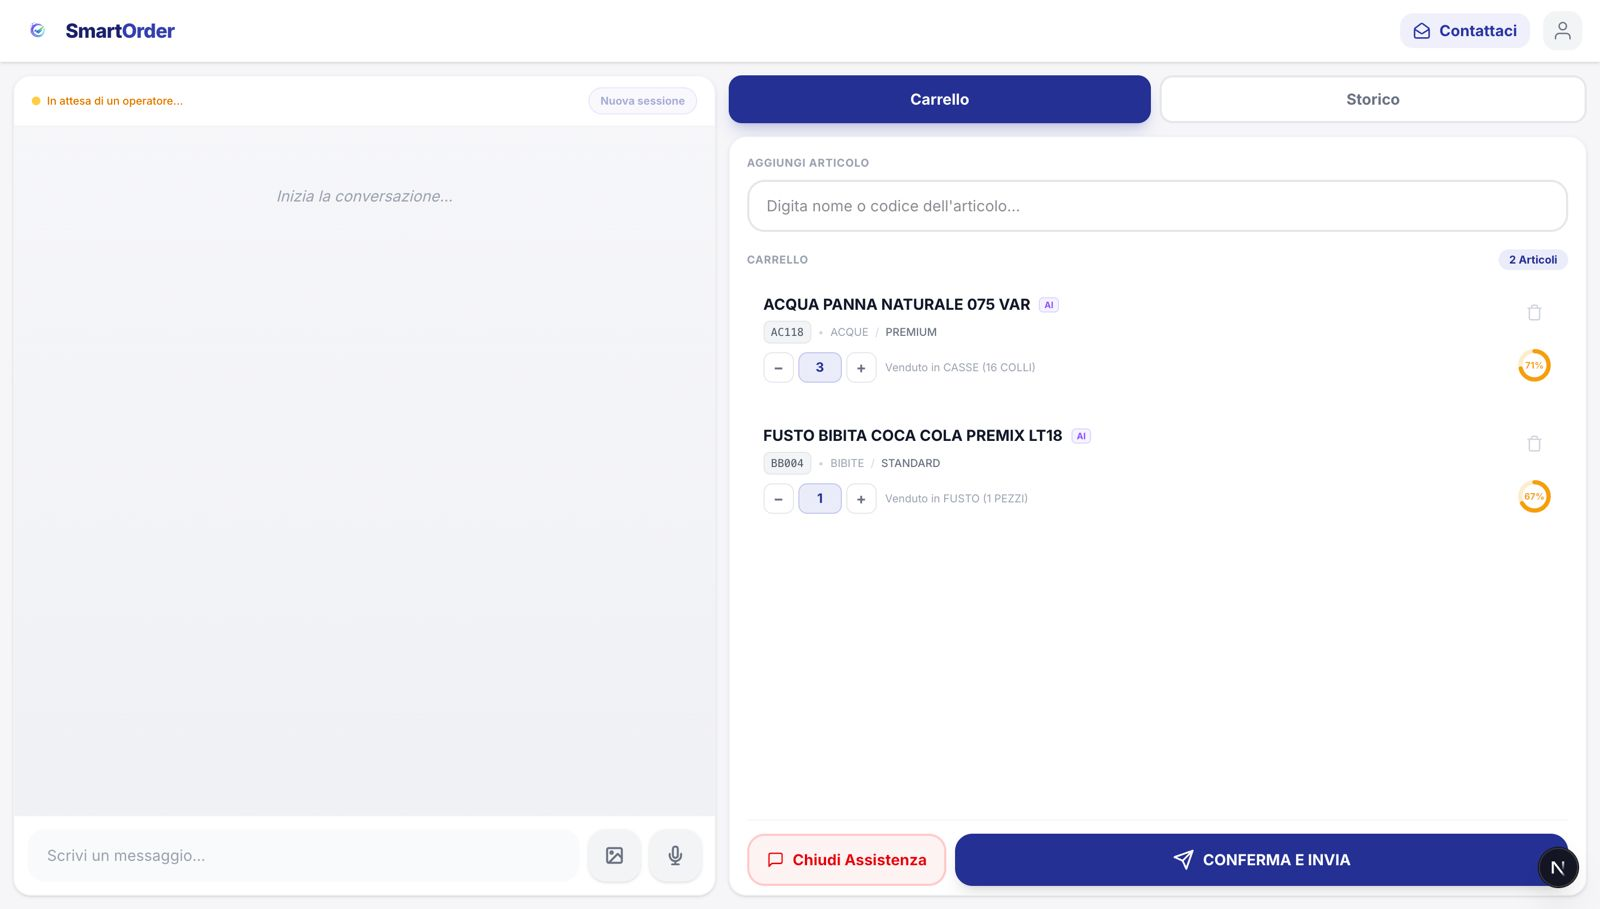
\includegraphics[width=0.7\textwidth]{Contenuti/immagini/ticket aperto.jpeg}
        \caption{Aspetto della chat dopo l'apertura di un ticket}
    \end{figure}

Per richiedere assistenza umana a un operatore:

\begin{enumerate}
    \item \textbf{Apertura}: Cliccare sul pulsante \texttt{Assistenza} nel pannello carrello (accanto a \texttt{CONFERMA E INVIA}).
    \item \textbf{Modale}: Si apre una finestra modale che mostra lo stato corrente dell'assistenza.
    \item \textbf{Nessun ticket attivo}: Se non ci sono ticket aperti, cliccare su \texttt{Richiedi Assistenza}. Viene creato un ticket e il sistema notifica un operatore.
    \item \textbf{Ticket esistente}: Se un ticket \`e gi\`a aperto, vengono mostrati lo stato (In attesa / In carico da un operatore) e, se gi\`a assegnato, il nome dell'operatore. \`E possibile chiudere il ticket con \texttt{Chiudi Assistenza}.
    \item \textbf{Chat con operatore}: Una volta aperto il ticket, la chat principale si trasforma: compare un banner \texttt{Chatta con l'operatore} e tutti i messaggi vengono instradati all'operatore assegnato. L'utente riceve le risposte dell'operatore in tempo reale tramite SSE. Il pulsante \texttt{Nuova sessione} rimane disabilitato finché il ticket \`e aperto.
\end{enumerate}

\subsection{Nuova sessione}

Per avviare una nuova conversazione:

\begin{enumerate}
    \item \textbf{Attivazione}: Cliccare sul pulsante \texttt{Nuova sessione} nella barra superiore del pannello chat. Il pulsante \`e disabilitato se \`e presente un ticket di assistenza aperto.
    \item \textbf{Conferma}: Viene visualizzata una finestra modale che chiede conferma: \texttt{La conversazione attuale e il carrello verranno cancellati. Vuoi procedere?}
    \item \textbf{Conferma / Annulla}: Premere \texttt{Conferma} per avviare una nuova sessione (chat e carrello vengono resettati) oppure \texttt{Annulla} per tornare alla sessione corrente.
\end{enumerate}

\subsection{Feedback}
    \begin{figure}[H]
        \centering
        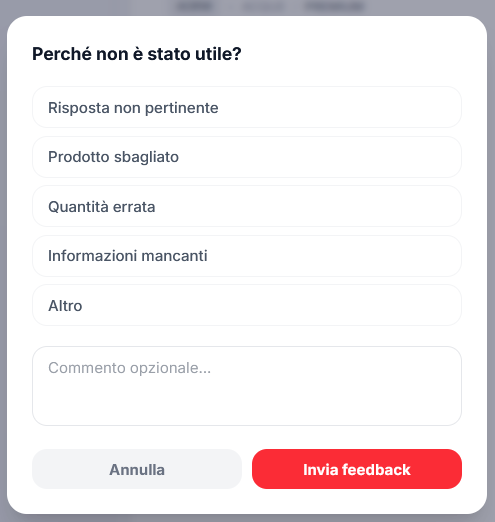
\includegraphics[width=0.4\textwidth]{Contenuti/immagini/feedback negativo.png}
        \caption{Dialogo per l'invio di un feedback negativo}
    \end{figure}
Per inviare un feedback sul messaggio generato dal chatbot è sufficiente premere uno dei due indicatori rappresentati da un pollice in su e un pollice in giù, per inviare dei feedback, rispettivamente, positivi o negativi.
In caso di feedback negativo è necessario indicare il motivo, con la possibilità di aggiungere un commento

\subsection{Area personale (Cliente)}

    \begin{figure}[H]
        \centering
        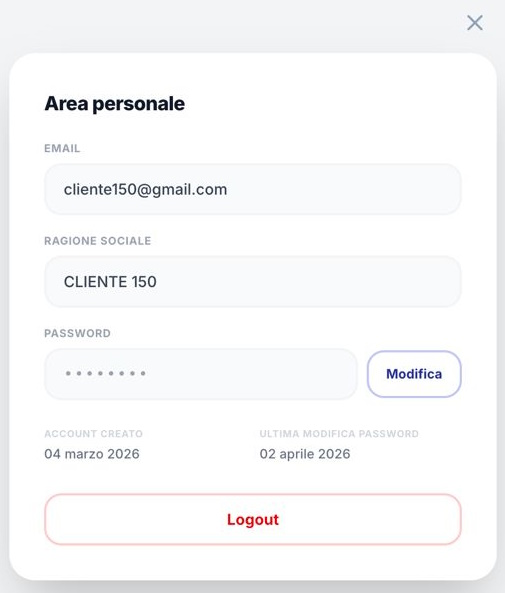
\includegraphics[width=0.4\textwidth]{Contenuti/immagini/area personale cliente finestra.jpg}
        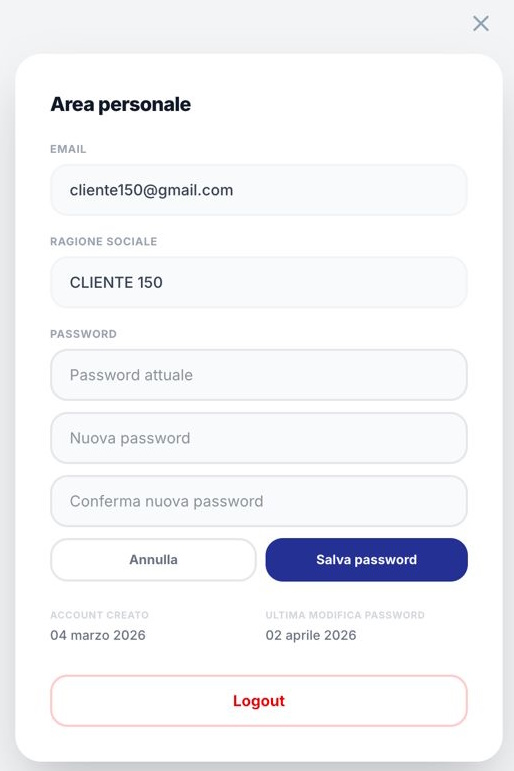
\includegraphics[width=0.4\textwidth]{Contenuti/immagini/cambio password cliente finestra.jpg}
        \caption{Area personale e cambio password}
    \end{figure}

Per accedere alle impostazioni del proprio profilo:

\begin{enumerate}
    \item \textbf{Apertura}: Cliccare sull'icona del profilo nella barra superiore destra.
    \item \textbf{Dati visibili}: Vengono mostrate le informazioni dell'account: email e ragione sociale.
    \item \textbf{Cambio password}: Cliccare su \texttt{Modifica} nella sezione password. Inserire la password attuale, la nuova password (minimo 6 caratteri) e confermarla. Premere \texttt{Salva password}.
    \item \textbf{Logout}: Cliccare sul pulsante \texttt{Logout} in fondo alla schermata per disconnettersi.
\end{enumerate}
